% Folding diagram for the Indonesian paper (paper_final_id/main_id.tex). English text so the figure can be reused.
% Compile: cd paper_final_id/figures && pdflatex fig_folding
\documentclass[border=2pt]{standalone}
\usepackage{amsmath,amssymb}
\usepackage{tikz}
\usetikzlibrary{positioning,arrows.meta,fit,calc}
\begin{document}
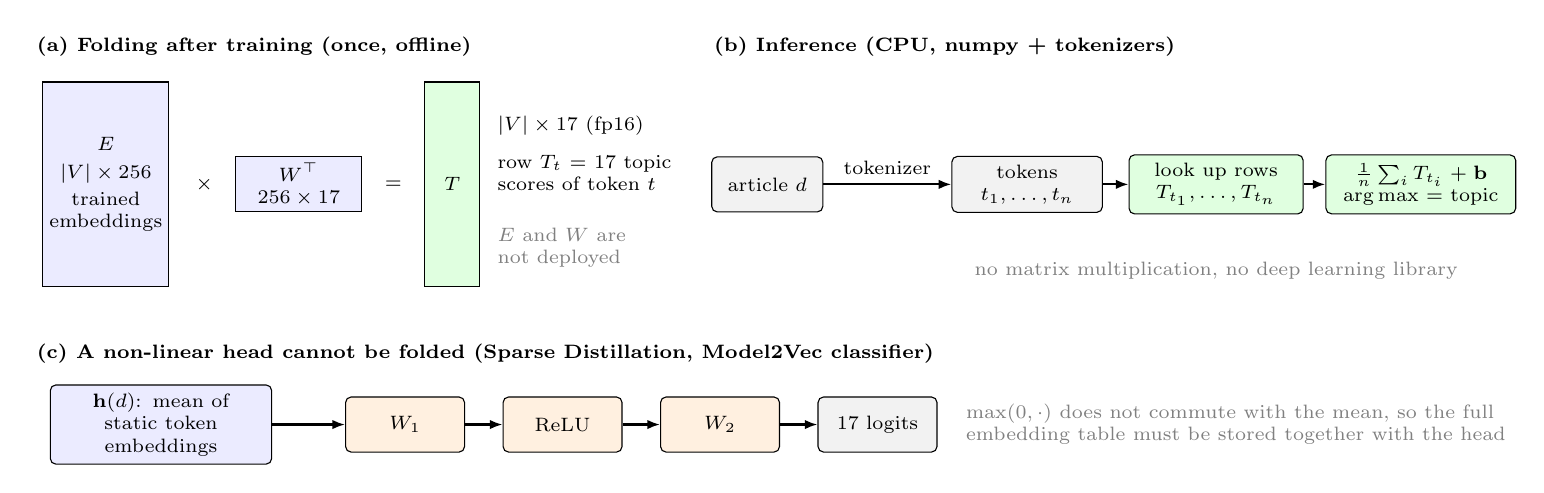
\begin{tikzpicture}[
  mat/.style={draw, align=center, font=\scriptsize, inner sep=2pt},
  box/.style={draw, rounded corners=2pt, align=center, font=\scriptsize, inner sep=3pt, minimum height=7mm},
  arr/.style={-{Latex[length=1.6mm]}, thick},
  lab/.style={font=\scriptsize},
  head/.style={font=\scriptsize\bfseries, anchor=west}]
  % ---------------- (a) folding after training ----------------
  \node[head] at (-0.2, 2.35) {(a) Folding after training (once, offline)};
  \node[mat, fill=blue!8, minimum width=16mm, minimum height=26mm] (E) at (0.8, 0.6) {$E$\\[2pt]$|V|\times 256$\\[2pt]trained\\embeddings};
  \node[lab] at (2.05, 0.6) {$\times$};
  \node[mat, fill=blue!8, minimum width=16mm, minimum height=7mm] (W) at (3.25, 0.6) {$W^{\top}$\\$256\times 17$};
  \node[lab] at (4.45, 0.6) {$=$};
  \node[mat, fill=green!12, minimum width=7mm, minimum height=26mm] (T) at (5.2, 0.6) {$T$};
  \node[lab, align=left, anchor=west] at (5.65, 1.35) {$|V|\times 17$ (fp16)};
  \node[lab, align=left, anchor=west] at (5.65, 0.75) {row $T_t$ = 17 topic\\scores of token $t$};
  \node[lab, align=left, anchor=west, text=gray] at (5.65, -0.2) {$E$ and $W$ are\\not deployed};
  % ---------------- (b) inference ----------------
  \node[head] at (8.4, 2.35) {(b) Inference (CPU, numpy + tokenizers)};
  \node[box, fill=gray!10, text width=12mm] (doc) at (9.2, 0.6) {article $d$};
  \node[box, fill=gray!10, text width=17mm] (tok) at (12.5, 0.6) {tokens\\$t_1,\dots,t_n$};
  \node[box, fill=green!12, text width=20mm] (look) at (14.9, 0.6) {look up rows\\$T_{t_1},\dots,T_{t_n}$};
  \node[box, fill=green!12, text width=22mm] (avg) at (17.5, 0.6) {$\frac{1}{n}\sum_i T_{t_i}+\mathbf{b}$\\$\arg\max$ = topic};
  \draw[arr] (doc) -- node[lab, above]{tokenizer} (tok);
  \draw[arr] (tok) -- (look);
  \draw[arr] (look) -- (avg);
  \node[lab, text=gray, align=center] at (14.9, -0.5) {no matrix multiplication, no deep learning library};
  % ---------------- (c) non-linear head ----------------
  \node[head] at (-0.2, -1.55) {(c) A non-linear head cannot be folded (Sparse Distillation, Model2Vec classifier)};
  \node[box, fill=blue!8, text width=26mm] (h) at (1.5, -2.45) {$\mathbf{h}(d)$: mean of\\static token embeddings};
  \node[box, fill=orange!12, text width=13mm] (w1) at (4.6, -2.45) {$W_1$};
  \node[box, fill=orange!12, text width=13mm] (relu) at (6.6, -2.45) {ReLU};
  \node[box, fill=orange!12, text width=13mm] (w2) at (8.6, -2.45) {$W_2$};
  \node[box, fill=gray!10, text width=13mm] (z) at (10.6, -2.45) {17 logits};
  \draw[arr] (h) -- (w1);
  \draw[arr] (w1) -- (relu);
  \draw[arr] (relu) -- (w2);
  \draw[arr] (w2) -- (z);
  \node[lab, align=left, anchor=west, text=gray] at (11.6, -2.45) {$\max(0,\cdot)$ does not commute with the mean, so the full\\embedding table must be stored together with the head};
\end{tikzpicture}
\end{document}
